\chapter{Synchronization Examples}
\section{POSIX Synchronization}

POSIX API proviedes:
\begin{itemize}
    \item mutex locks
    \item semaphores
    \item condition variable
\end{itemize}

Widely used on UNIX, Linux, and macOS.

\section{POSIX Mutex Locks}

Creating and initializing the lock

\begin{codeInC}
#include <pthread.h>

pthread_mutex_t mutex;

/* create and initialize the mutex lock */
pthread_mutex_init(&mutex, NULL);

\end{codeInC}

Acquiring and releasing the lock

\begin{codeInC}
/* acquire the mutex lock */
pthread_mutex lock (&mutex);

/* critical section */

/* release the mutex lock */
pthread_mutex_unlock(&mutex);
\end{codeInC}

\newpage
\section{POSIX Semaphores}

POSIX provides two versions – \textbf{named} and \textbf{unnamed}. Named semaphores can be used by unrelated processes, unnamed
cannot, similar to named / unnamed pipes.

\subsection{POSIX Named Semaphores}
Creating an initializing the semaphore:

\begin{codeInC}
#include <semaphore.h>
sem_t *sem;

/* Create the semaphore and initialize it to 1 */
sem = sem_open("SEM", O_CREAT, 0666, 1);

\end{codeInC}

Another process can access the semaphore by referring to its name SEM


\paragraph{}
Acquiring and releasing the semaphore:
\begin{codeInC}
/* acquire the semaphore */
sem_wait(sem);

/* critical section */

/* release the semaphore */
sem_post(sem);

\end{codeInC}


\subsection{POSIX Unnamed Semaphores}

Creating an initializing the semaphore:

\begin{codeInC}
#include <semaphore.h>

sem_t sem;

/* Create the semaphore and initialize it to 1 */
sem_init(&sem, 0, 1);

\end{codeInC}

Acquiring and releasing the semaphore:

\begin{codeInC}
/* acquire the semaphore */
sem_wait(&sem);

/* critical section */

/* release the semaphore */
sem_post(&sem);

\end{codeInC}

\newpage
\section{POSIX Condition Variables}

Since POSIX is typically used in C/C++ and these languages do not
provide a monitor, POSIX condition variables are associated with a
POSIX mutex lock to provide mutual exclusion: Creating and initializing
the condition variable:


\begin{codeInC}
#include <pthread.h>

pthread_mutex_t mutex;
pthread_cond_t cond_var;

/* Initialize the mutex lock and condition variable */
pthread_mutex_init(&mutex, NULL);
pthread_cond_init(&cond_var, NULL);

\end{codeInC}
\paragraph{}
Thread waiting for the condition a == b to become true:

\begin{codeInC}
pthread_mutex_lock(&mutex);
while (a != b)
    pthread_cond_wait(&cond_var, &mutex);
    
pthread_mutex_unlock(&mutex);

\end{codeInC}

Thread signaling another thread waiting on the condition variable:

\begin{codeInC}
pthread_mutex_lock(&mutex);
a = b;
pthread_cond_signal(&cond_var);
pthread_mutex_unlock(&mutex);
\end{codeInC}

\paragraph{NOTE: } pthread\_cond\_wait unlocks the mutex just before it sleeps, but then it re-acquires the
mutex (which may require waiting) when it is signalled, before it wakes up.
So if the signalling thread holds the mutex (the usual case), the waiting thread will not
proceed until the signalling thread also unlocks the mutex.
\paragraph{}
\textbf{This can generate a deadlock!} 

\newpage
\section{Java Synchronization}
Java creates an entry queue that contains the threads that want to access the critical section. Java provides rich set of synchronization features:

\begin{itemize}
    \item Java monitors
    \item Reentrant locks
    \item Semaphores
    \item Condition variables
\end{itemize}

Every Java object has associated with it a single lock.

\begin{itemize}
    \item[] If a method is declared as synchronized, a calling thread must own the lock for the object.
    \item[] If the lock is owned by another thread, the calling thread must wait for the lock until it is released.
\end{itemize}

Locks are released when the owning thread exits the synchronized method.

\begin{codeInJava}
public class BoundedBuffer<E> {

  private static final int BUFFER_SIZE = 5;

  private int count, in, out;
  private E[] buffer;

  public BoundedBuffer() {
    count = 0;
    in = 0;
    out = 0;
    buffer = (E[]) new Object[BUFFER_SIZE];
  }

  /* Producers call this method */
  public synchronized void insert(E item) {
    // ...
  }

  /* Consumers call this method */
  public synchronized E remove() {
    // ...
  }
}

\end{codeInJava}

A thread that tries to acquire an unavailable lock is placed in the
object’s entry set:

\begin{figure}[htbp]
    \centering
    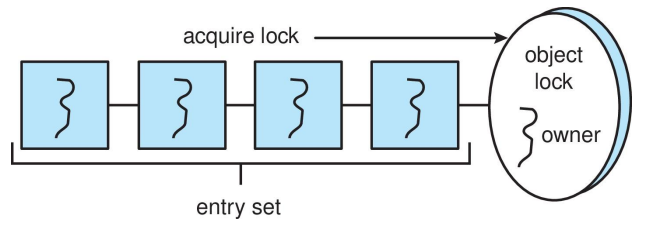
\includegraphics[width=0.42\linewidth]{img/advcasdv.png}
\end{figure}

Similarly, each object also has a wait set.
\newpage
When a thread calls wait():

\begin{enumerate}
    \item It releases the lock for the object
    \item The state of the thread is set to blocked
    \item The thread is placed in the wait set for the object
\end{enumerate}

\begin{figure}[htbp]
    \centering
    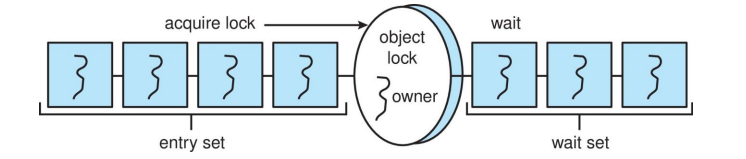
\includegraphics[width=0.65\linewidth]{img/adavasd.png}
\end{figure}


A thread typically calls \textbf{wait()} when it is waiting for a condition to
become true.

But the question is: how does a thread get notified?
\paragraph{}

When a thread calls \textbf{notify()}:

\begin{itemize}
    \item An arbitrary thread T is selected from the wait set;
    \item T is moved from the wait set to the entry set;
    \item Set the state of T from blocked to runnable.
\end{itemize}
T can now compete for the lock to check if the condition it was waiting for is now true.

\subsection{Java Semaphores}

Constructor:

\begin{codeInJava}
Semaphore(int value);
\end{codeInJava}

Usage:

\begin{codeInJava}
Semaphore sem = new Semaphore(1);

try{

    sem.acquire();

    /* Cristical section */

}catch (InterruptedException ie) {
    // do something
}finally{
    sem.release();
}
\end{codeInJava}

\newpage
\section{OpenMP Synchronization}
OpenMP is a set of compiler directives and API that support
parallel progamming.

\begin{codeInC}
void update(int value){

    #pragma omp critical
    {
        count += value
    }
 }
\end{codeInC}

\paragraph{NOTE: } the curly brackets must be in a new line.

The code after the \verb|#pragma omp critical| contains a critical section and it will be performed atomically.


\section{Bounded buffer}

The bounded-buffer problems, a.k.a. the producer-consumer problem, is a classic example of concurrent access to a shared
resource. A bounded buffer lets multiple producers and multiple
consumers share a single buffer. 

\begin{itemize}
    \item[] Producers write data to the buffer and consumers read data from the buffer.
    \item[] Producers must block if the buffer is full.
    \item[] Consumers must block if the buffer is empty
\end{itemize}

\begin{figure}[htbp]
    \centering
    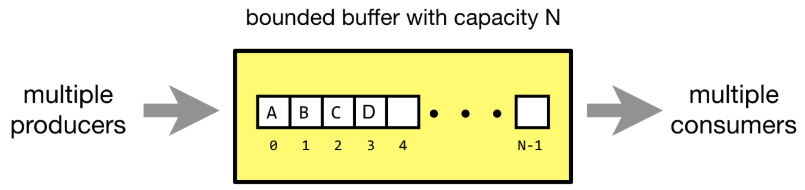
\includegraphics[width=0.5\linewidth]{img/pc_problem.png}
\end{figure}

How can we solve the problem with semaphores?

\begin{enumerate}
    \item Semaphore mutex initialized to the value 1, to avoid concurrent accesses to the buffer;
    \item Semaphore elements initialized to the value 0, to know if there is something to read;
    \item Semaphore free initialized to the value n to track free spaces.
\end{enumerate}

The structure of the producer process:

\begin{codeInC}
while (true) {
         ...
         /* produce an item in next_produced */
         ...
     wait(free);
     wait(mutex);
         ...
         /* add next produced to the buffer */
         ...
     signal(mutex);
     signal(elements);
 }
\end{codeInC}


The structure of the consumer process:

\begin{codeInC}
while (true) {
     wait(elements);
     wait(mutex);
         ...
         /* remove an item from buffer to next_consumed */
         ...
     signal(mutex);
     signal(free);
         ...
         /* consume the item in next consumed */
         ...
 }
\end{codeInC}


\section{Readers-Writers Problem}
A data set is shared among a number of concurrent processes:

\begin{itemize}
    \item Readers – only read the data set; they do not perform any updates
    \item Writers – can both read and write
\end{itemize}

Problem – allow multiple readers to read at the same time, only one single writer can access the shared data at the same
time.


\begin{figure}[htbp]
    \centering
    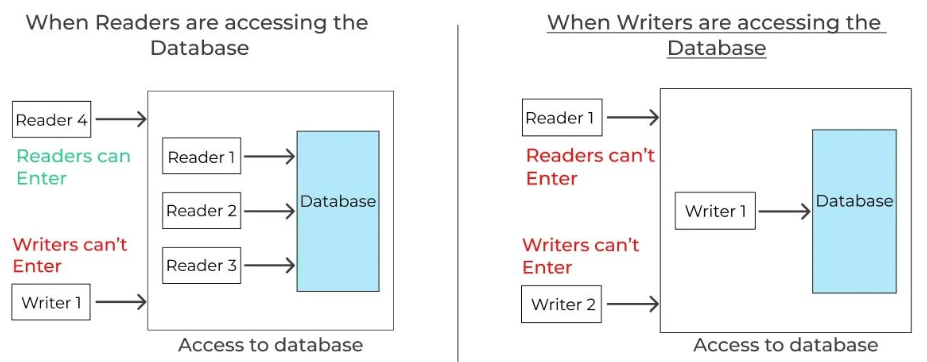
\includegraphics[width=0.85\linewidth]{img/read_asd.png}
\end{figure}

\paragraph{}
We want to access into a shared data: Data set, how we can do?

\begin{itemize}
    \item Semaphore rw\_mutex initialized to 1, this is to deal with the fact that there should not be two writers or a reader and a writer at the same time
    \item Integer read\_count initialized to 0, this is to keep track of how many readers are there
    \item Semaphore mutex initialized to 1, this is to update read\_count safely
\end{itemize}

\newpage
The structure of a writer process

\begin{codeInC}
while (true) {
    wait(rw_mutex);
        ...
        /* writing is performed */
        ...
    signal(rw_mutex);
}
\end{codeInC}

The structure of a reader process


\begin{codeInC}
while (true){
    wait(mutex);
    read_count++;
    if (read_count == 1) // first reader needs lock
        wait(rw_mutex);
    signal(mutex);
    ...
    /* reading is performed */
    ...
    wait(mutex);
    read_count--;
    if (read_count == 0) // last reader releases lock
        signal(rw_mutex);
    signal(mutex);
}
\end{codeInC}

There are some problems:
The solution can result in a situation where
a writer process never writes. It is referred to as the “First
reader-writer” problem.

\paragraph{}
The “Second reader-writer” problem is a variation the first
reader-writer problem that state: Once a writer is ready to write, no “newly arrived
reader” is allowed to read.

\paragraph{}
Both the first and second may result in \textbf{starvation}. Leading to
even more variations. The problem is solved on some systems by kernel providing
\textbf{reader-writer locks}.

\newpage
\section{Dining-Philosophers Problem}

This is a conceptual problem. N philosophers’ sit at a round table with a bowel of rice in the middle

\begin{figure}[htbp]
    \centering
    
\includegraphics[width=0.3\linewidth]{img/phil.png}
\end{figure}

Each philosopher to eat must take the right and the left chopstick. But if everyone take before the left chopstick, none can eat and it produce a starvation.
\paragraph{}
In the case of 5 philosophers, the shared data
\begin{itemize}
    \item Bowl of rice (data set)
    \item Semaphore chopstick [5] initialized to 1
\end{itemize}

Semaphore Solution, the structure of Philosopher i :

\begin{codeInC}
while (true){
    wait (chopstick[i] );
    wait (chopStick[ (i + 1) \% 5] );
    
        /* eat for awhile */
        
    signal (chopstick[i] );
    signal (chopstick[ (i + 1) \% 5] );
    
        /* think for awhile */
}
\end{codeInC}

There is a problem: if each philosopher takes the i-th chopstick and then waits
for the other they can not! \textbf{DEADLOCK}.

Easy solution: one philosopher behaves asymmetrically, willing
to take the i+1-th chopstick first.

\newpage
\subsection{Monitor Solution to Dining Philosophers}


\begin{codeInC}
monitor DiningPhilosophers{
    enum {THINKING; HUNGRY, EATING} state [5];
    condition self [5];
    
    void take_fork (int i) {
        state[i] = HUNGRY;
        test(i);
        if (state[i] != EATING)
        self[i].wait;
    }
    void put_fork (int i) {
        state[i] = THINKING;
        // test left and right neighbors
        test((i + 4) \% 5);
        test((i + 1) \% 5);
    }
    void test (int i) {
        if ((state[(i + 4) \% 5] != EATING) && (state[i] == HUNGRY) &&(state[(i + 1) \% 5] != EATING) ) {
            state[i] = EATING ;
            self[i].signal () ;
        }
    }
    initialization_code() {
        for (int i = 0; i < 5; i++)
            state[i] = THINKING;
    }
}
\end{codeInC}

Each philosopher “i” invokes the operations take\_fork() and
put\_fork() in the following sequence:

\begin{codeInC}
DiningPhilosophers.take_fork(i);
    /** EAT **/
DiningPhilosophers.put_fork(i);
\end{codeInC}

No deadlock, but starvation is possible.